%!TEX program = xelatex

% Name           : hsrm-beamer-minimal.sty
% Author         : Benjamin Weiss (benjamin.weiss@kreatiefton.de)
% Version        : 0.2
% Created on     : 08.05.2013
% Last Edited on : 24.03.2014
% Copyright      : Copyright (c) 2013 by Benjamin Weiss. All rights reserved.
% License        : This file may be distributed and/or modified under the
%                  GNU Public License.
% Description    : HSRM beamer theme minimal example.

\documentclass{beamer}

%\usepackage[german]{babel}
\usepackage[english]{babel}
\usepackage{multirow}
\usepackage{rotating}


%% MATH -----------------------------------------------------------
\newcommand{\modulo}[1]{\vert#1\vert}
\newcommand{\norm}[1]{\left\Vert#1\right\Vert}
\newcommand{\abs}[1]{\left\vert#1\right\vert}
\newcommand{\set}[1]{\left\{#1\right\}}
\newcommand{\Real}{\mathbb R}
\newcommand{\eps}{\varepsilon}
\newcommand{\To}{\longrightarrow}
\newcommand{\BX}{\mathbf{B}(X)}
\newcommand{\A}{\mathcal{A}}
\newcommand{\Cero}{\mathbf 0}


\usetheme{hsrm}

\title{MVFCMddV and Multiclasification.}
\subtitle{Projeto AM 2016-1}
\author{Pedro Diamel Marrero Fernandez \\ Juan González Hidalgo }
\institute{Universidade Federal de Pernambuco\\Brasil {\Medium CIn}}
\date{\today}

\begin{document}

\maketitle

\section*{Topics}
\begin{frame}
	\frametitle{Topics}
	\tableofcontents[hideallsubsections]
\end{frame}

\section{Introduction}

\begin{frame}{Topics}	
\begin{itemize}
\item MVFCMddV: A multi-view relational fuzzy c-medoid vectors clustering algorithm. Neurocomputing, 163, 115-123.de Carvalho, F. D. A. and others.
\begin{itemize}
\item Synthetic data.
\item Real data.
\item Application in image compress.
\end{itemize}
\item Multiclassifier System.
\begin{itemize}
\item Real data.
\end{itemize}

\end{itemize}
\end{frame}


\section{Result}



\begin{frame}{MVFCMddV synthetic data}

Data generate:

\begin{figure}[h]
\centering
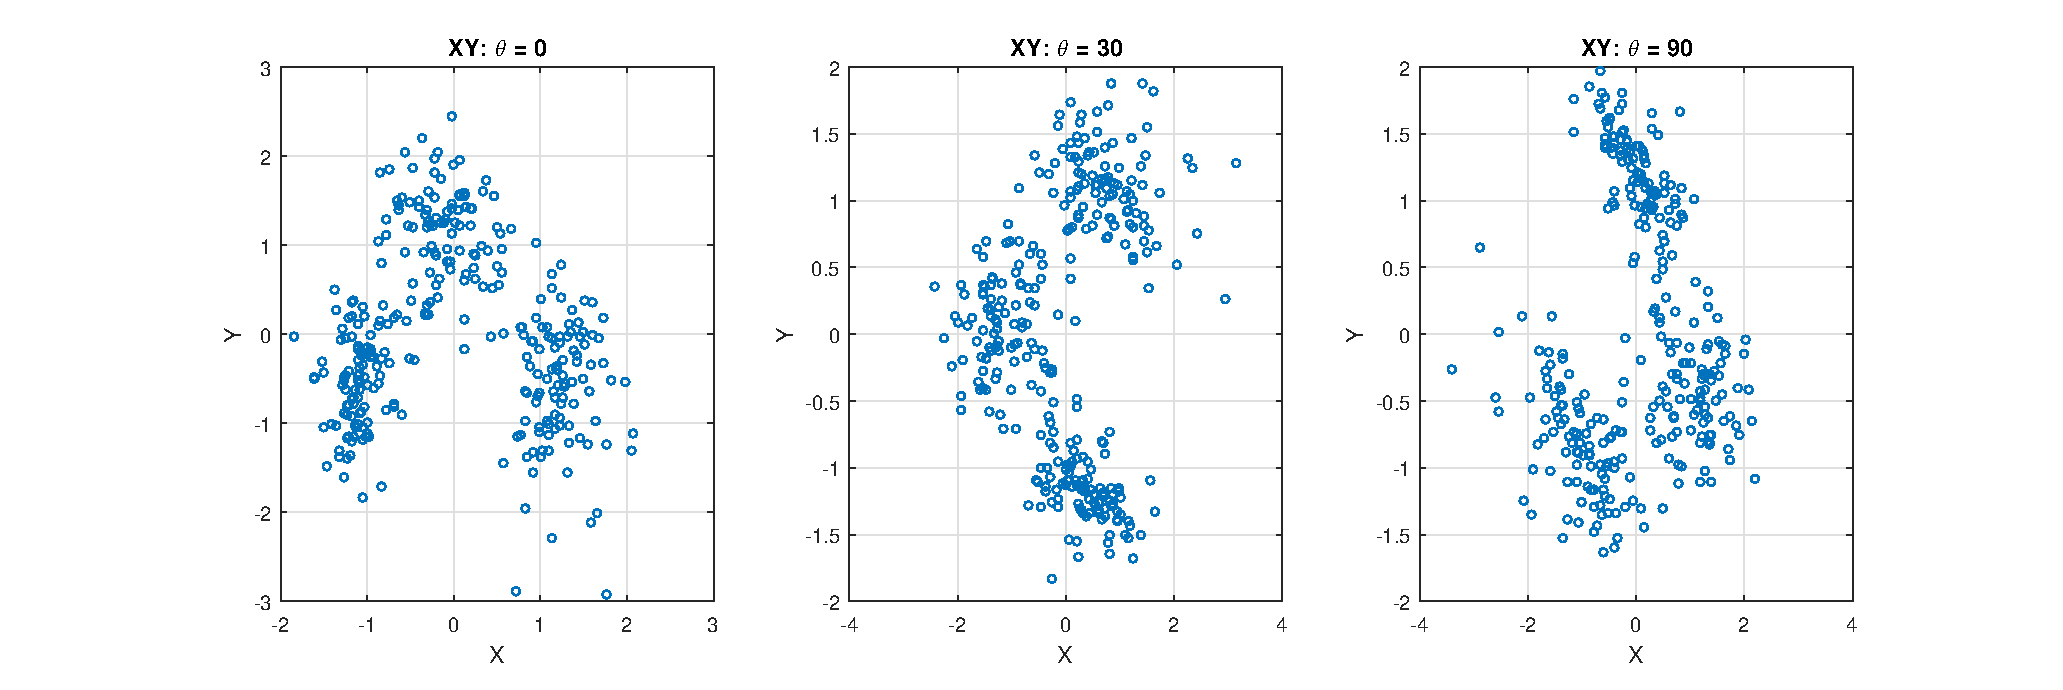
\includegraphics[width=4.5in]{../out/xy-sinteticos.eps}
\caption{Synthetic data generate.}
\label{fig:xy_sinteticos}
\end{figure}  

\end{frame}

\begin{frame}{MVFCMddV synthetic data}

Configuration method input: $K = 3$, $m = 1.2$, $T = 10$, $\epsilon = 1e^{-500}$.
Result: Corrected Rand Index (CR) de $0.98$.
\begin{figure}[h]
\centering
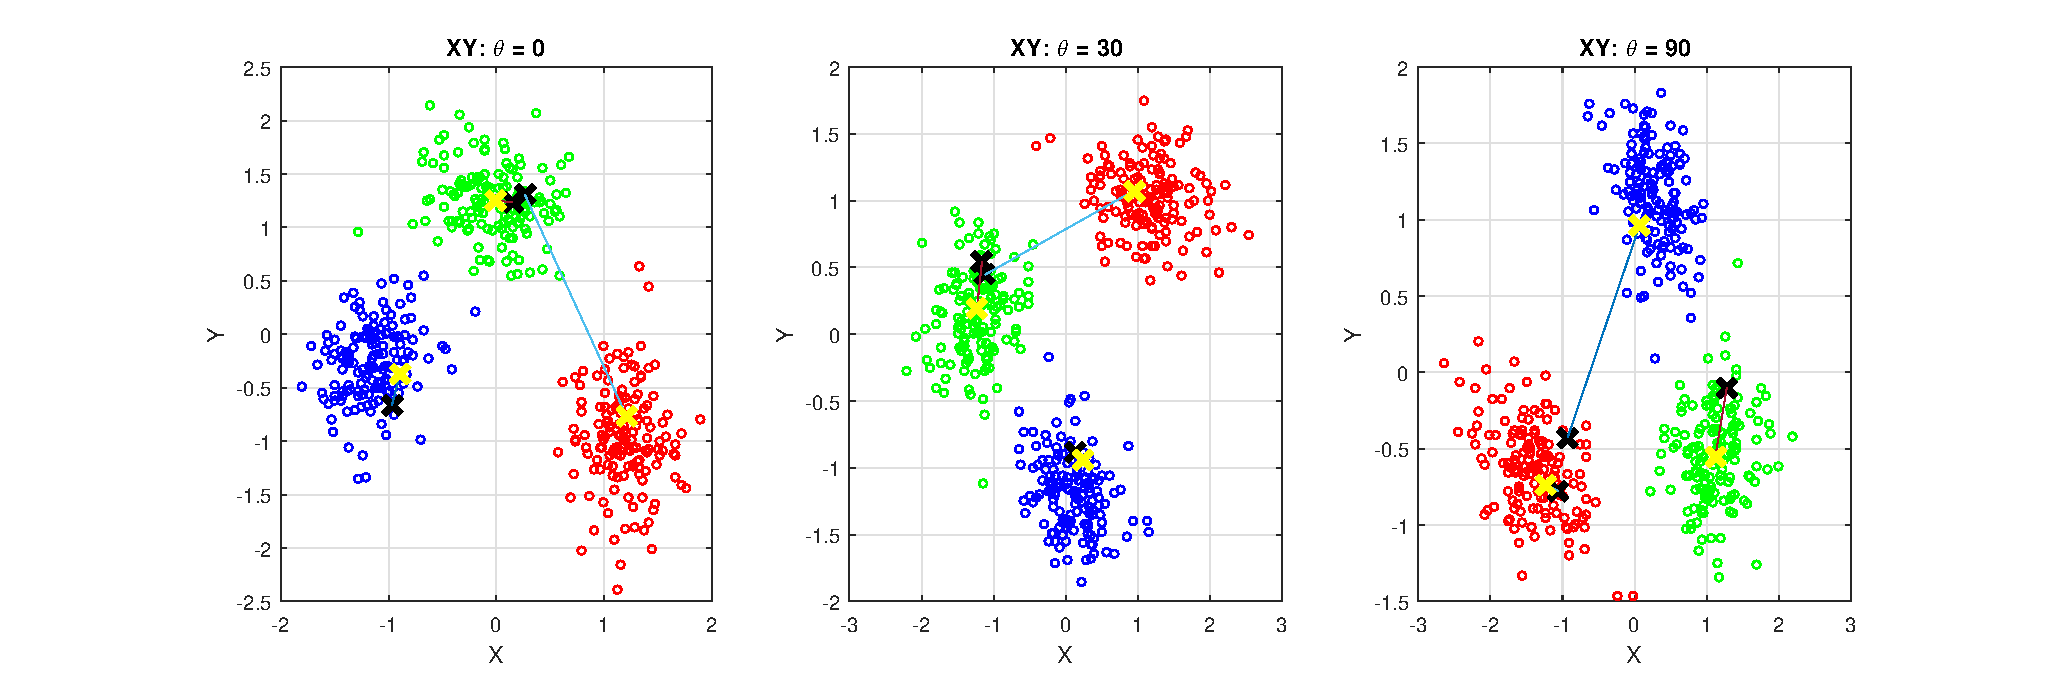
\includegraphics[width=4.5in]{../out/clusters-gauss-3.eps}
\caption{Clustering hard for MVFCMddV.}
\label{fig:cluster_datos_sinteticos}
\end{figure}  

\end{frame}


\begin{frame}{MVFCMddV real data}
\begin{figure}[h]
\centering
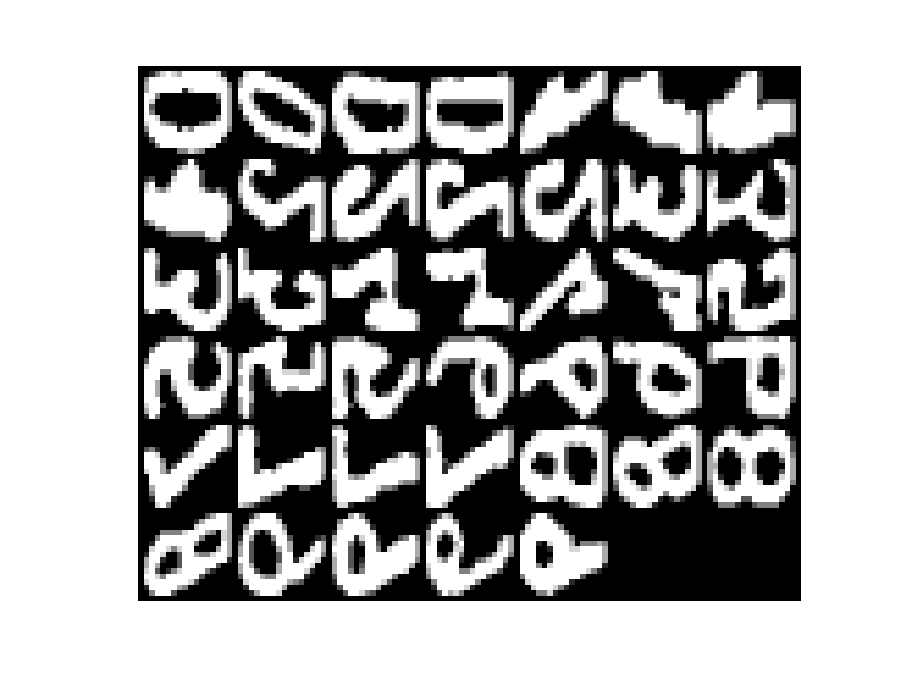
\includegraphics[width=3.0in]{../out/data-base.eps}
\caption{Multiple Features Data Set.}
\label{fig:data_base}
\end{figure}  
\end{frame}

\begin{frame}{MVFCMddV real data}
\begin{enumerate}
\item \textbf{mfeat-fout: (FOUT)} 76 Fourier coefficients. ***
\item \textbf{mfeat-fac (FAC):} 216 profile correlations.
\item \textbf{mfeat-kar (KAR):} 64 Karhunen-Loève coefficients. ***
\item \textbf{mfeat-pix (PIX):} 240 pixel averages in 2 x 3 windows.
\item \textbf{mfeat-zer (ZER):} 47 Zernike moments. ***
\item \textbf{mfeat-mor (MOR):} 6 morphological features.
\end{enumerate}
\end{frame}

\begin{frame}{MVFCMddV real data}
Configuration method input:
$K =10$, $m = 1.6$, $T = 150$, $\epsilon = 1e^{-10}$, $N = 100$.
\begin{figure}[h]
\centering
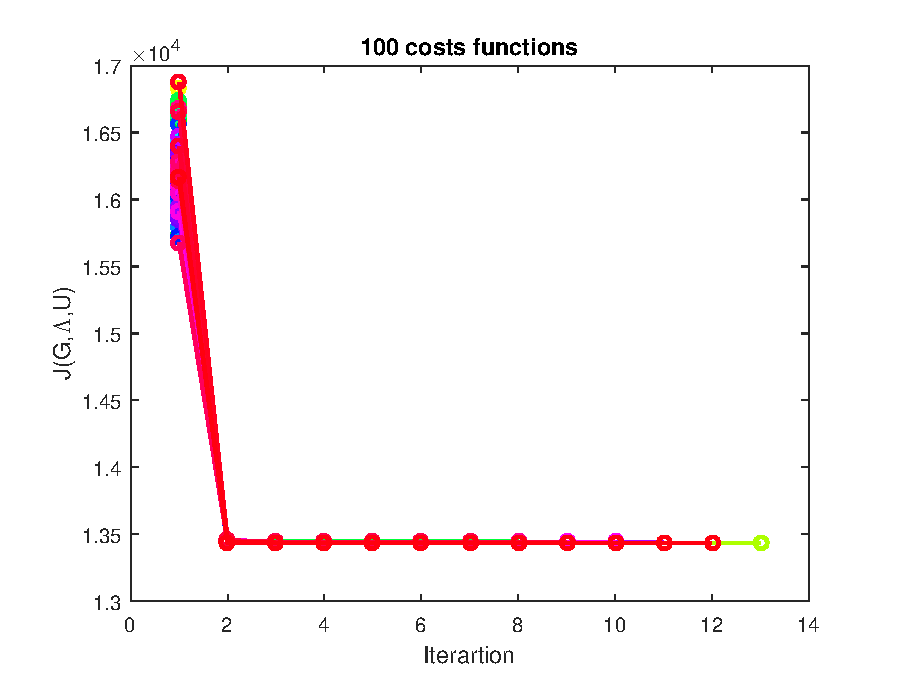
\includegraphics[width=2.5in]{../out/cost-function-mvfcmddv.eps}
\caption{MVFCMddV in 100 iterations.}
\label{fig:data_base}
\end{figure}
\end{frame}

\begin{frame}{MVFCMddV real data}
Result: 
\begin{itemize}
\item Corrected Rand Index (CR): $0.108$.
\item F-mesure: $0.345$. 
\end{itemize}
\end{frame}


\begin{frame}{MVFCMddV application in image compress}
\begin{figure}[h]
\centering
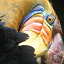
\includegraphics[width=2.0in]{../out/bird_small.png} 
\caption{Original image of $64 \times 64$. The size in pixeles is iqual to  $64\times64\times3\times8 = 98.304$ }
\label{fig:lab}
\end{figure}
\end{frame}


\begin{frame}{MVFCMddV application in image compress}
\begin{figure}[h]
\centering
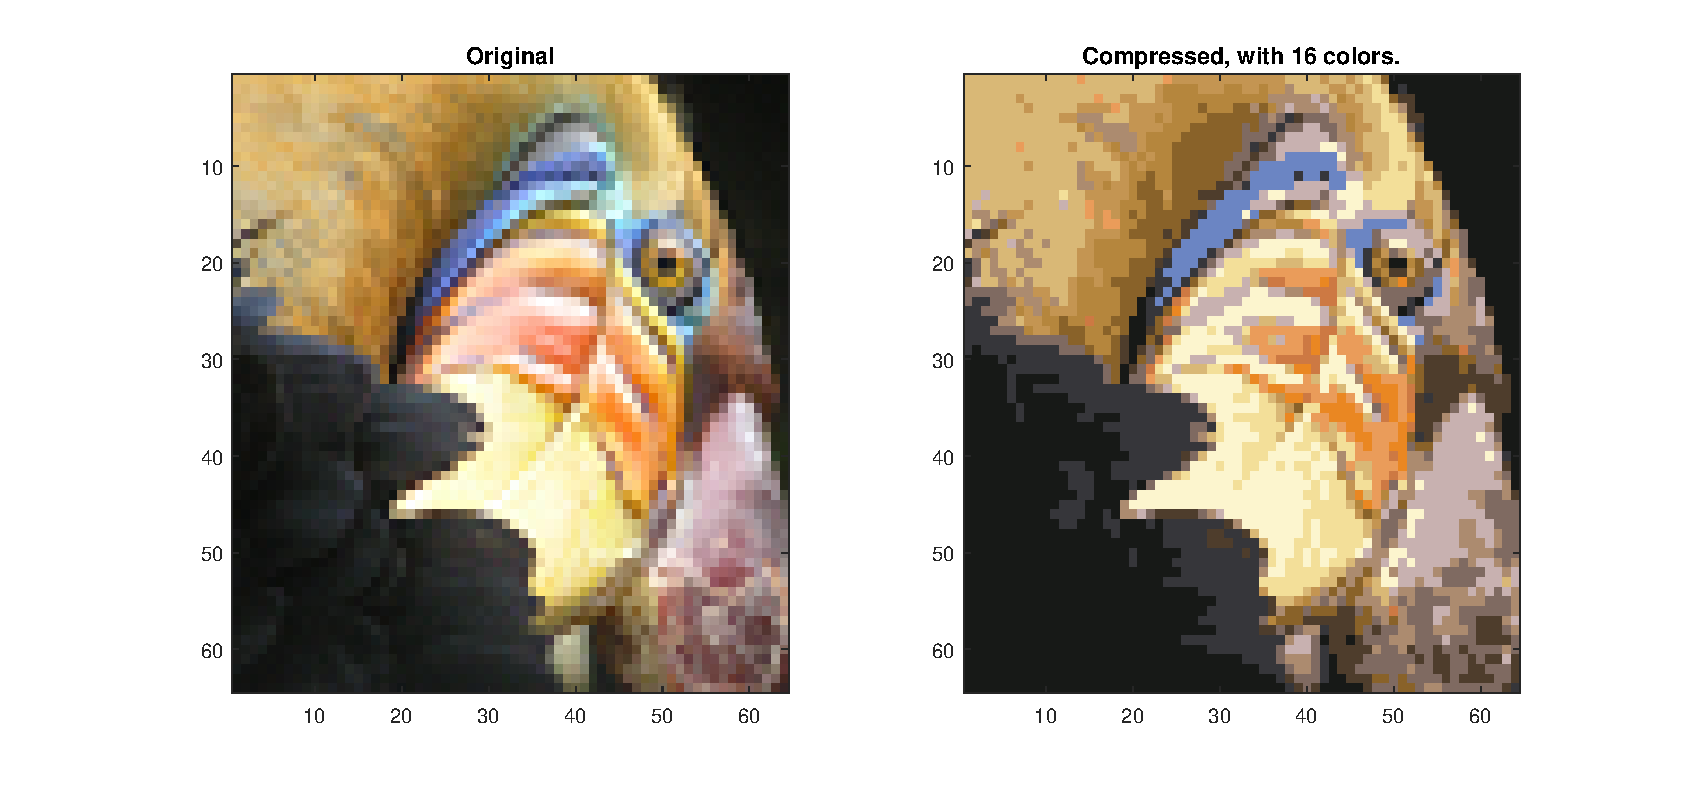
\includegraphics[width=4.5in]{../out/image-compress-16.eps}
\caption{Image raw vs image compress. The size in pixel the image compress is $16\times24 + 64\times64\times4 = 16.384$}
\label{fig:image_compress}
\end{figure}
\end{frame}




\begin{frame}{Multiclassifier System}
\begin{figure}[h]
\centering
\includegraphics[width=3.0in]{../out/system-multclassy.eps}
\caption{Multiclassifier System architecture.}
\label{fig:mult_system_classy}
\end{figure}  
\end{frame}

\begin{frame}{Multiclassifier System}
\begin{itemize}
\item Data base: Multiple Features Data Set.
\item Validate: 40-kfold cross-validation (Training, Validation and Test sets).
\item Models: Bayes, SVM, MLP. 
\item Parameters: $C$, $\lambda$.
\end{itemize}
\end{frame}


\begin{frame}{Multiclassifier System}
\begin{figure}[!h]
\centering
\begin{tabular}{cc}
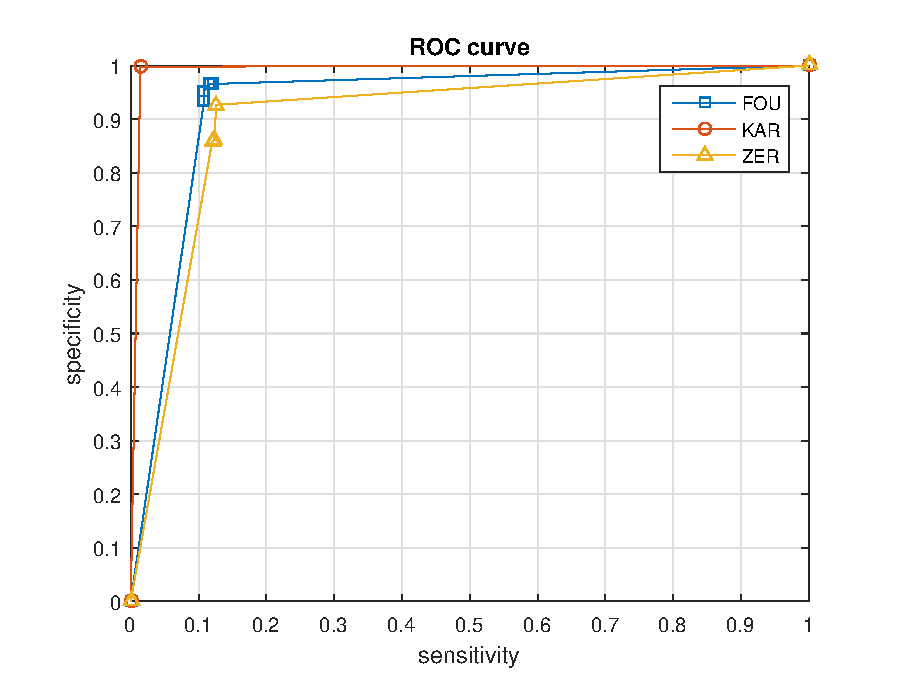
\includegraphics[width=2.0in]{../out/svm-roc.eps}&
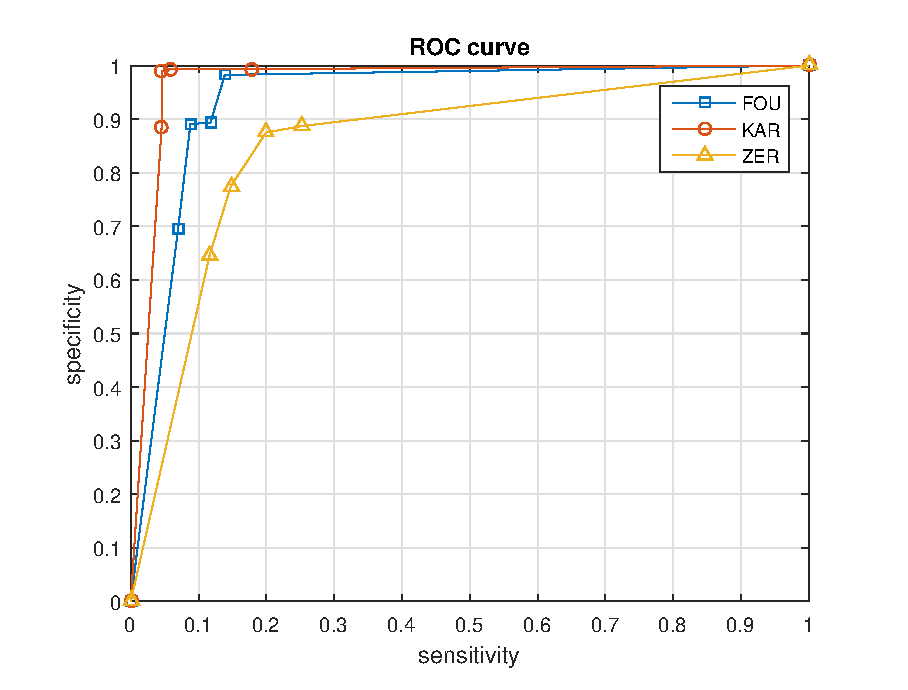
\includegraphics[width=2.0in]{../out/mlp-roc.eps} \\
a) SVM  & b) MLP
\end{tabular}
\caption{ROC curve.}
\label{fig:roc_curve}
\end{figure}
\end{frame}




\begin{frame}{Multiclassifier System}
\begin{table}[!h]
\renewcommand{\arraystretch}{1.3}
\caption{Summary.}
\label{tab:analisis_data}
\centering
\scalebox{0.7}{
\begin{tabular}{c}
\begin{tabular}{rcccc}
\hline
         &B   &     SVM  &  MLP   &  COMB     \\
\hline     
 Min.    &0.800   &0.860   &0.860   &0.860\\  
 1st Qu. &0.880   &0.900   &0.895   &0.900\\  
 Median  &0.900   &\textbf{0.920}   &\textbf{0.920}   &\textbf{0.920}\\  
 Sd      &0.037   &0.035   &0.032   &0.034\\
 Mean    &0.901   &0.920   &0.915   &0.926\\  
 3rd Qu. &0.920   &0.940   &0.940   &0.960\\  
 Max.    &0.980   &0.980   &0.980   &0.980\\  
\hline 
\end{tabular}\\
\multicolumn{1}{p{2.8in}}{B: Classificador Bayesiano, SVM: Máquina de Vetor de Suporte, MLP:Perceptron Multi-camadas, COMB: Regra de Combinação pelo Voto Maioritario.}
\end{tabular}}
\end{table} 
\end{frame}

\begin{frame}{Multiclassifier System}
\begin{figure}[h]
\centering
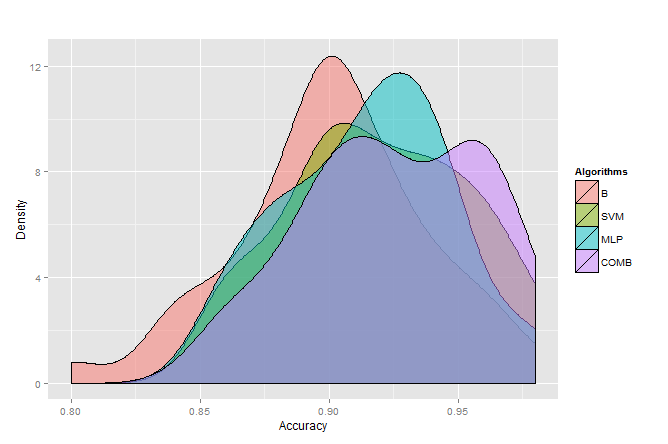
\includegraphics[width=3.5in]{../out/density-graph.png} \\
\caption{Grafico de densidade das amostras correspondentes à saída do erro de cada método testado.}
\label{fig:densidade_acc}
\end{figure} 
\end{frame}


\begin{frame}{Multiclassifier System}
\begin{figure}[!h]
\centering
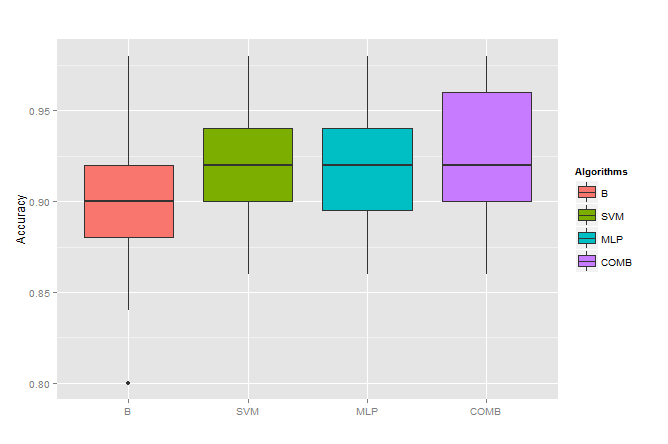
\includegraphics[width=3.5in]{../out/boxplot-errors.png}
\caption{Box plot dos métodos avaliados.}
\label{fig:boxplot_acc}
\end{figure} 
\end{frame}


\begin{frame}{Multiclassifier System}
Adherence test for combination methods: 
\begin{enumerate}
\item $H_0$: is normal distribution
\item $H_1$: not normal distribution
\item $\alpha = 0.05$
\item Lilliefors (Kolmogorov-Smirnov) normality test
\item p-value = 0.006916
\item The hypothesis $H_0$ is reject.
\end{enumerate}
\end{frame}


\begin{frame}{Multiclassifier System}
Hypothesis test:
\begin{enumerate}
\item $H_0$: $\ M_1 = M_2 = ... =M_n$
\item $H_1$: $\exists M_i,M_j \ | \ M_i\neq M_j$
\item $\alpha = 0.05$
\item ANOVA Friedman test
\item p-value = 0.0002
\item The hypothesis $H_0$ is reject.
\end{enumerate}
\end{frame}


\begin{frame}{Multiclassifier System}
\begin{table}[!h]
\renewcommand{\arraystretch}{1.3}
\caption{Teste de Comparação Múltiple de Nemenyi }
\label{tab:test_nemeyi}
\centering
\scalebox{0.7}{
\begin{tabular}{c}
\begin{tabular}{rccc}
\hline
    &B       &SVM     &MLP         \\    
\hline                             
SVM &0.06497 &-       &-           \\  
MLP &0.07245 &0.99997 &-           \\
COMB &\textbf{0.00047} &0.45437 &0.42808    \\
\hline 
\end{tabular}\\
\multicolumn{1}{p{2.8in}}{ B: Classificador Bayesiano, SVM: Máquina de Vetor de Suporte, MLP: Perceptron Multi-camadas, COMB:  Regra de Combinação pelo Voto Maioritario.}
\end{tabular}}
\end{table}
\end{frame}

\begin{frame}{Multiclassifier System}
Conclusion:


\end{frame}



\begin{frame}{Conclusion}
\begin{itemize}
\item ...
\end{itemize}
\end{frame}

\begin{frame}{}
Thank you...
\end{frame}


\end{document}






